%!TEX root = proj_report_outline.tex
\chapter{Threshold Security Scheme}\label{C:threshholdSecurity}
This chapters discusses the importance of database security, introduces threshold security schemes and describes how Shamir's Secret Sharing scheme has been integrated with PitchHub for the purposes of fulfilling design requirement D2.3: The prototype must store sensitive data securely.

\section{Database Security}\label{S:databaseSecurity}
Securely storing data is a large and increasingly important research area to modern society. In recent years companies like Sony, Apple and Adobe have experienced data breaches resulting in compromised user data. In a system like PitchHub where commercially sensitive information is being handled extreme care must be taken to ensure its safety. 

\subsection{Background into Threshold Security Schemes}
Secret Sharing schemes are a type of Threshold Security Scheme where a piece of data is split into \textit{n} secret shares. To retrieve the original data a threshold of \textit{k} of \textit{n} shares ("\textit{k}, \textit{n}") must be met before the original piece of data can be decrypted. A fictional scenario that describes this concept is where the code for launching a nuclear missile is split between three officers, to launch the missile all three officers must be present to reconstruct the launch code. Each share in isolation cannot be used to launch the missile, nor can it be used to infer the original code. This "3, 3" example is somewhat contrived but it showcases the fundamentals of secret sharing in that: the secret can be recovered given the threshold is met and the secret is indeed secret given any combination of \textit{t} shares less than \textit{k}.

\subsection{Shamir's Secret Sharing Scheme}
Shamir's secret sharing \cite{shamir1979share} is a threshold scheme based on polynomial interpolation. 

\[q(x) = a_o +a_1x + ... + a_{k-1}x^{k-1} \]

The fundamental idea is that given a "\textit{k}, \textit{n}" scheme a random polynomial of degree \textit{k}-1 may be generated where the secret \textit{D} is hidden as term \(a_o\). A set of \textit{n} points may then be constructed from this polynomial and shared to \textit{n} secret keepers. To recover the secret \textit{D} the process requires a subset of \textit{k} secret shares to calculate the coefficients of the polynomial using interpolation. With this a system is able to recover the secret \textit{D} at term \(a_o\).
\par
Shamir's Secret Sharing scheme effectively allows a system to share secrets to \textit{n} secret keepers while maintaining each secret's safety as a long as a threshold of \textit{k} malicious secret keepers is not met. Besides being secure, Shamir's Secret Sharing scheme holds a number of other useful properties such as being minimal, extensible and dynamic \cite{shamir1979share}. The scheme is minimal in that the the size of each share does not exceed the size of the original secret. The scheme is extensible in that \textit{n} may be increased by giving new secret keepers new points from the polynomial. The scheme is dynamic in that the shares may be changed by modifying the polynomial but retaining the term \(a_o\).
\par
As discussed in a number studies the simplicity of Shamir's Secret Sharing scheme does present limitations that have the potential for being exploited \cite{abdallah2015analysis}\cite{dautrich2012security}. First, complete trust is given to the system who is dealing the secret shares, if an error occurs the secret may be irrecoverable therefore the system dealing the shares can be seen as a single point of failure. Second, Shamir's Secret Sharing scheme cannot detect secret keepers that cheat by supplying wrong shares, this brings about the problem where if \textit{k} members are compromised not only will the secrets be recoverable by the malicious party but the compromised members may be used to supply wrong secret shares to the system, effectively denying the first party system of recovering secrets. To combat these exploits Shamir's Secret Sharing may be extended with signature schemes \cite{shoup2000practical}\cite{abdalla2001forward} and verification schemes that do not assume the party dealing the shares is honest or infallible \cite{herzberg1995proactive}\cite{cachin2002asynchronous}.

\section{Security Design}
In this section discussion is presented on how Shamir's Secret Sharing scheme has been implemented into the PitchHub prototype.

\subsection{Shamir's Secret Sharing Scheme Service}\label{SS:design_shamir_secret_sharing_service}
The first action in designing the service was choosing an open-source implementation of Shamir's Secret Sharing. Deciding to use an open-source implementation over writing a custom implementation was a key design decision. While the principles of Shamir's Secret Sharing are simple, personally implementing a cryptography library should be treated with care. To implement and establish trust in such a component would require rigorous testing to be proven as secure. Leveraging the collective strength of the open-source community ensures that the implementations have had many eyes go through them (with different backgrounds/expertises). The primary activity for PitchHub in regards to Secret Sharing was to design and implement a service that integrates the security scheme.
\par
As discussed by prominent cryptographer and author \citeauthor{schneier1999cryptography} ``Building cryptography into products is hard... Flaws can appear anywhere. They can be in the trust model, the system design, the algorithms and protocols, the implementations, the source code, the human-computer interface, the procedures, the underlying computer system. Anywhere.'' \cite{schneier1999cryptography}. PitchHub  approached the integration of the security scheme library with emphasis on limiting the amount of coupling. By reducing coupling between the library and wider system we reduce the risk of system knowledge producing vulnerabilities within PitchHub and undermining the security scheme's integrity.
\par
In designing this service the MVC architecture pattern was analysed in regards to which component is most suitable to handle this responsibility. The model could use a Ruby mixin to override both it's \textit{save} and \textit{find} methods such that the secret was split into \textit{n} shares on \textit{save} for the \textit{n} databases. \textit{Find} would work similarly, merely combining the queried shares from the \textit{k..n} databases and presenting the clear text secret. The view component is not supposed to deal with business logic and hence not an appropriate candidate for this responsibility. The controller in it's capacity of delegating tasks to models could also bear this responsibility. In the controller on \textit{saves} it could split the secret among \textit{n} models and save each model to a distinct database. With \textit{finds} the controller would need to connect to each database and retrieve the requested secrets to combine. The pros and cons of each design is apparent. Going strictly the model route would mean \textit{monkey patching} \cite{Monke1:online} the behaviour of the ODM which could make it hard for other components that do not wish to use the Secret Sharing implementation also this would require that models have knowledge outside of itself. Going strictly controller means that there is a fair amount of business logic within the controllers. However, both approaches consolidate the integration of the Secret Sharing library within it's own component. Ultimately, the final approach was a mixture of the above, controllers were modified such that they use explicit Secret Sharing \textit{find} and \textit{save} methods which encapsulate the knowledge of the \textit{n} secret keeper databases, within these explicit Secret Sharing database methods the logic of the Secret Sharing library is isolated.
\par
Despite both Models and Controllers being aware of the Secret Sharing functionality, they are only aware of as much to the capacity of their roles. The model handles the business logic, while the controller handles the delegation.

\subsection{Overcoming Limitations of Threshold Security Schemes}
Given share combinations up to \textit{k}, Secret Sharing Schemes ensure that the secret's safety is maintained. However, if an attacker gains \textit{k} secret shares, the secret is easily reconstructed. This is simultaneously the advantage and weakness of Threshold Security Schemes. To explore further in the context of PitchHub: up to \textit{k} compromised databases do not compromise the security of the secrets being held, but if an attacker is able to break into one database it is reasonable to infer that they are capable of breaking into all of them. Furthermore this scheme relies on the availability of \textit{k} secret keepers, should \textit{k} be unattainable the secrets are rendered irretrievable to both authorised and unauthorised users alike.
\par
The first issue can be alleviated by introducing diversity to the secret keepers. Instead of all secret keepers being MongoDB instances including alternative data stores in the secret keeper configuration means that the vulnerabilities of the data stores themselves do not manifest as a vulnerability for the system as a whole. However, to do this effectively we require a configuration where there is not \textit{k} secret keepers of the same data store. If there were, the whole exercise of including alternative data stores would be rendered moot as an attacker with the ability to breach the particular data store would be able to fulfil the threshold \textit{k}. This issue of diversity and security is explored by \citeauthor{littlewood2004redundancy} who conclude that depending on the context diversity can be one of the most effective means of neutralising `systemic' attacks by merely avoiding the danger.
\par
There is a fundamental tension in the relationship between availability and security in threshold schemes. Representations of the classic Threshold Security Schemes where each secret keeper contains one and only share of the secret favour security over availability. This is great when secret keepers do not have any membership changes or only member changes that still preserve \textit{k} secret keepers. In this example should \textit{k} or more secret keepers go down the entire service becomes unavailable, and in cases where \textit{k} cannot ever be re-established then the secret data is irretrievable. There are a number of approaches that can be used to increase availability but each suffer from an increase in complexity and a decrease in security. For example, concepts used in distributed databases are directly applicable to secret sharing schemes. Redundancy and hinted hand-off are methods used by distributed database systems are used to ensure availability by node's sharing their data such that if they go down the data stored is still accessible through the nodes who hold the shared data. In the context of Threshold Schemes this means that some nodes may have more than one secret share for the same secret, this demonstrably reduces the significance of the threshold. For a system like PitchHub I believe classic redundancy, where each member contains a whole other keeper's secret shares, is a step too far. Instead I suggest raising the availability of the secret members themselves by representing secret members as high availability (HA) replica sets rather than individual database instances, this architecture configuration is featured in Fig \ref{fig:architecture_high_availability}.

\begin{figure}[ht]
    \centering
    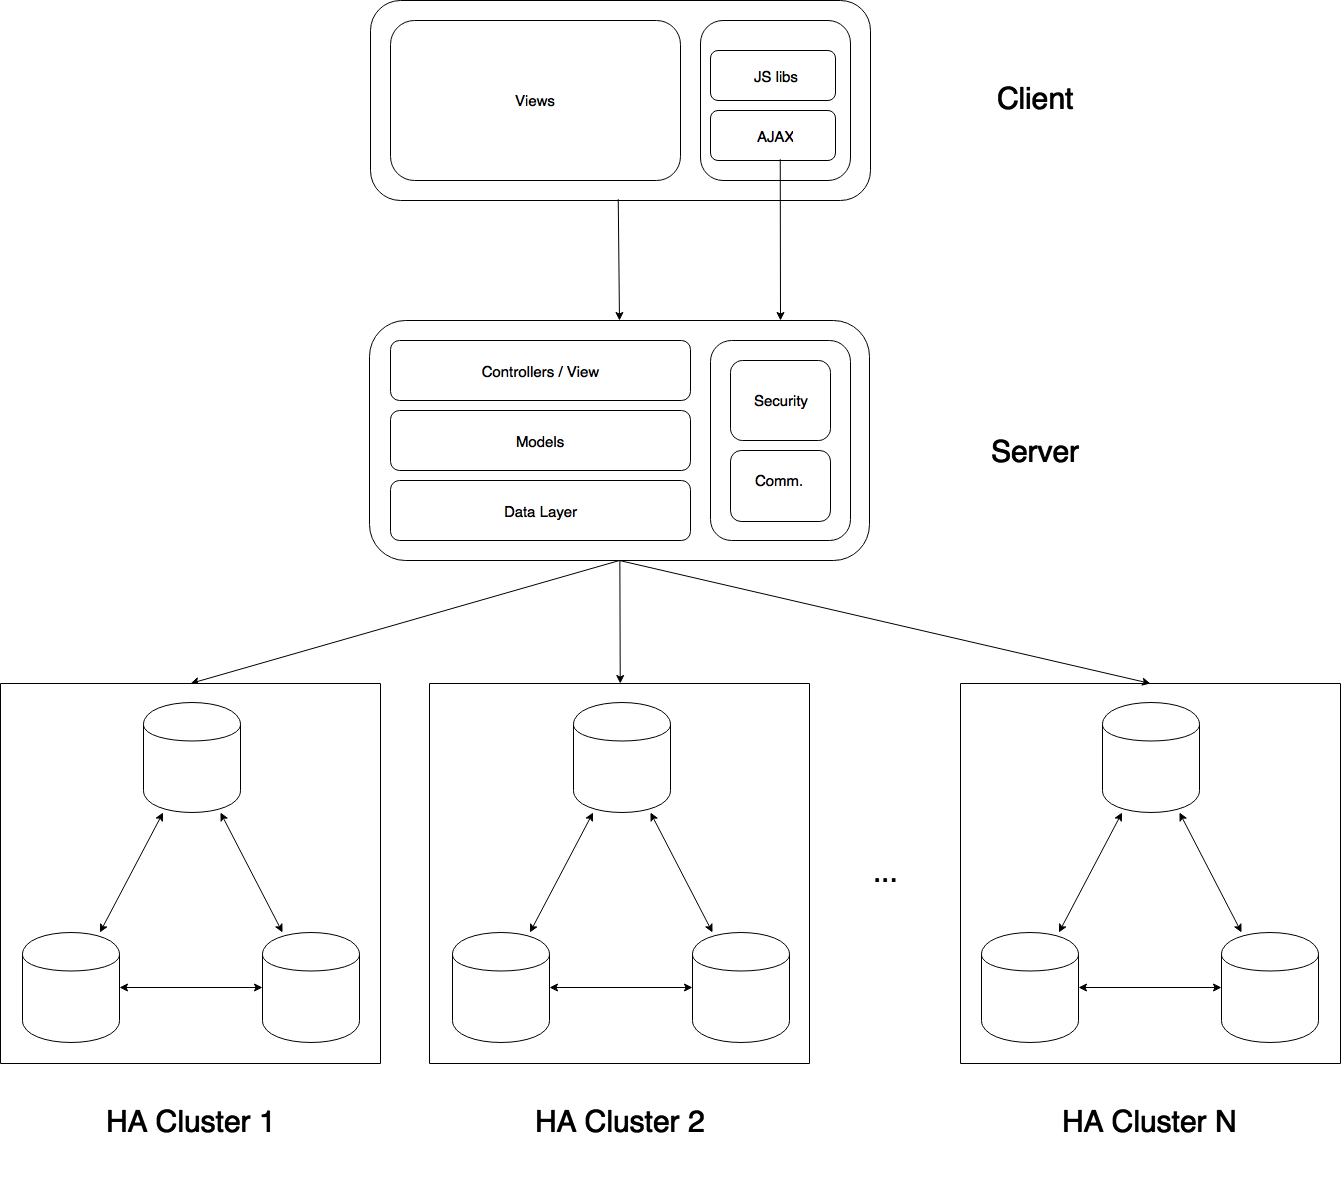
\includegraphics[width=1\textwidth]{architecture_high_availability}
    \caption{The architecture extended with high-availability (HA) replica sets increases the Threshold Scheme's robustness without compromising security.}
    \label{fig:architecture_high_availability}
\end{figure}

\section{Implementation}

\subsection{Shamir's Secret Sharing Scheme Service}
Beyond the configuration of the service which is further explored in Subsection \ref{SS:diverse_secret_keepers} an initial concern was in determining at what granularity the Pitch Cards/Contribution objects should be split. The options considered were as follows: split a binary representation of the object, split each field present in the object, or split only the sensitive fields in the object. The first option results in the entire object being encrypted with little ability to reason about the contents. This approach is considered too restrictive as data such as \textit{user id}, \textit{status}, and \textit{timestamps} would have to be exposed to facilitate meaningful database queries. The second approach is better with regard to the fact that the structure of the data is reflected in the database however we would still require the same exposing of attributes as the first option. Ultimately, the approach for splitting objects was done on the field level, where each object's sensitive values are split and then placed into a new share that is persisted. Fig \ref{fig:comment_split} visualises how this done on a comment object. 

\begin{figure}[ht]
    \centering
    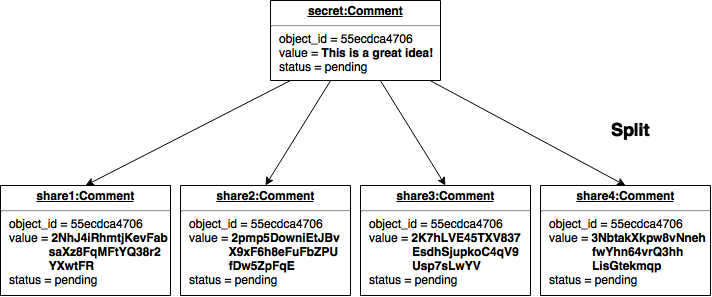
\includegraphics[width=1\textwidth]{comment_split}
    \caption{A comment object shown before and after the split operation. Each secret share contains an indecipherable portion of the original secret.}
    \label{fig:comment_split}
\end{figure}

\subsection{Diverse Secret Keepers}\label{SS:diverse_secret_keepers}

The secret sharing configuration developed for the prototype used a (\textit{3},\textit{4})-threshold scheme, where at least 3 of the 4 shares representing a secret must be combined to reconstruct the secret. The technologies used for the Secret Keepers are as follows: 2x MongoDB instances, and 2x PostgreSQL instances. The motivation behind using PostgreSQL instances to diversify the Secret Keepers is twofold. First, as discussed in Subsection \ref{SS:databaseSelection} the relational model is the ideal way to model N:M relationships users have with Pitch Cards and Suggestions/Comments. Second, the relational model is supported as the primary object-mapping system by Ruby on Rails. Given these reasons there are an abundance of advantages: modelling the data in a natural way that fits it's structure, better support throughout the development of the component, ability to prototype at a high velocity. Consideration was given to other document-model solutions such as CouchDB \cite{Apach2:online} and Couchbase \cite{Accel4:online} however these proved to have an underwhelming level of documentation for their ODM libraries.
\par
An initial concern was that the upfront schema set-up and overall schema-strictness required by relational databases would impact PitchHub's portability and extensibility, important attributes captured in requirement \textit{F4}. Thankfully, Ruby on Rails has out-of-the-box support for \textit{migrations} which enable database schemas to be defined/altered incrementally. This is another case of PitchHub configuring infrastructure in code and opening the door for automation.
\par
The most manual portion of setting up PitchHub at this stage is that the migrations required being manually executed on each database instance (as well as maintaining separate configuration files for each instance). To consolidate and automate this process PitchHub leverages the open-source community's \textit{Octopus} library \cite{tchan7:online}. Octopus enables sharding and migration management for distributed database configurations. Integrating Octopus restores near `plug-and-play' functionality. Still required is the actual setting up of the PostgreSQL instances. This can be done manually or via Vagrant but even this is considered to violate requirement \textit{F4}, which identifies non-technical users being able to easily set up a local instance of PitchHub. To resolve this issue, the (development branch of) PitchHub makes use of SQLite \cite{SQLit5:online}, a self-contained SQL database. This configuration while not appropriate for production makes local instances of PitchHub with the secret sharing configuration easily accessible by non-technical users.













